% This is LLNCS.DEM the demonstration file of
% the LaTeX macro package from Springer-Verlag
% for Lecture Notes in Computer Science,
% version 2.4 for LaTeX2e as of 16. April 2010
%
\documentclass{llncs}
\pagestyle{plain}  % switches on printing of running heads
%
\usepackage{makeidx}  % allows for indexgeneration
\usepackage{graphicx}
\usepackage{pgf}
\usepackage{tikz}
\usepackage{wasysym}
\usepackage{listings}
\usepackage[]{algorithm2e}
\usepackage{caption}

\usetikzlibrary{arrows,automata,positioning}

%
\begin{document}
	
%
\frontmatter          % for the preliminaries
%

\begin{titlepage}
	
\vspace*{4cm}

\begin{center} 
	
\textsc{\LARGE University of Bayreuth}\\[1.5cm]

\textsc{\LARGE Bachelor Seminar Tree Automata}\\[0.5cm]

% Title
\newcommand{\HRule}{\rule{\linewidth}{0.5mm}}
\HRule \\[0.4cm]
{	\huge \bfseries Introduction to Ranked Tree Automata\\[0.4cm] }
\HRule \\[1.5cm]

% Author and supervisor
\begin{minipage}{0.4\textwidth}
	\begin{flushleft} \large
		\emph{Author:}\\
		Martin \textsc{Braun}
	\end{flushleft}
\end{minipage}
\hfill
\begin{minipage}{0.4\textwidth}
	\begin{flushright} \large
		\emph{Supervisor:} \\
		Prof. Dr. Wim \textsc{Martens}
	\end{flushright}
\end{minipage}

\end{center}

\end{titlepage}

\newcommand{\nfaExample}{
	 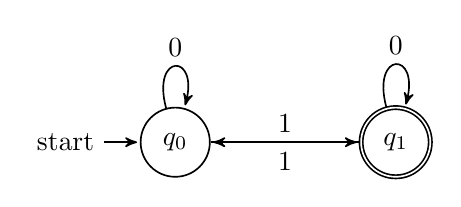
\begin{tikzpicture}[->,>=stealth',shorten >=1pt,auto,node distance=2.8cm,
                 		   semithick]
 				\tikzstyle{every state}=[fill=white,draw=black,text=black]
		
				\node[initial,state]		(A)			{$q_0$};
				\node[state,accepting]	(B)	[right of=A]	{$q_1$};
	
 				 \path (A)	edge	[loop above]	node {0}	(A)
					(A)	edge			node {1}	(B)
					(B)	edge	[loop above]	node {0}	(B)
					(B)	edge			node {1}	(A);
	\end{tikzpicture}
}

\newcommand{\moveStar}{\rightarrow_A^*}
\newcommand{\moveStarDet}{\rightarrow_{A_d}^*}

\newcommand{\simpleTreeExample} {
	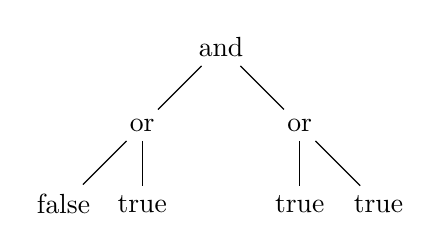
\begin{tikzpicture}[auto]
	\node (and) at (2, 3) {and};
	\node (or1) at (1, 2) {or};
	\node (or2) at (3, 2) {or};
	\node (false1) at (0, 1) {false};
	\node (true1) at (1, 1) {true};
	\node (true2) at (3, 1) {true};
	\node (true3) at (4, 1) {true};
	
	\draw [-] (and) to (or1);
	\draw [-] (and) to (or2);
	\draw [-] (or1) to (false1);
	\draw [-] (or1) to (true1);
	\draw [-] (or2) to (true2);
	\draw [-] (or2) to (true3);
	\end{tikzpicture}
}


\chapter*{Introduction to Tree Languages}
A good example for a tree language is the one consisting of all binary boolean expressions evaluating to true, for which an instance - if formatted in the right way - could look like this:

\begin{center}
	\(and(or(false, true), or(true, true))\)\\
\end{center}
To simplify, the elements of the language are often represented as a tree in a graphical way:
\begin{center}
	\simpleTreeExample
\end{center}
~\\
Just like for regular word languages, it is of interest to know whether a given word (in this case a tree) is part of the (tree-)language. In order to describe an automaton that recognizes tree-languages we have to define what \textbf{\(\Sigma\)-trees} and (regular) \textbf{tree-languages} are, first.

\begin{definition}{\(\Sigma\)-tree \cite{automata-xml}}
	\\
	The set of \(\Sigma\)-trees \(T_\Sigma\) over the \textbf{alphabet \(\Sigma\)} is inductively defined as follows:
	\begin{center}
		1. every \(\sigma \in \Sigma\) is a \(\Sigma\)-tree\\
		2. \(\sigma \in \Sigma\) and \(t_1,...,t_n \in T_\Sigma, n \ge 1 \iff \sigma(t_1,...,t_n) \in T_\Sigma\) 
	\end{center}
\end{definition}
~\\
\textit{Note: In general, there is no bound for the number of children in a tree (these trees are called \textit{unranked}), but in this paper we will only take a look at \textbf{ranked trees}, which have such a bound.}

\begin{definition}{tree-language \cite{automata-xml}}
	\\
	A tree language \(L_{t\Sigma}\) over the alphabet \(\Sigma\) is defined as a subset of \(T_\Sigma\):
	\begin{center}
		\(L_{t\Sigma} \subseteq T_\Sigma\)
	\end{center}	
\end{definition}

From that definition, we can see that \(T_\Sigma\) is already a tree-language.
Next, we have to declare some terminology in the context of $\Sigma-trees$.

\pagebreak
We can now define (Non-Deterministic) Finite Tree Automata for tree languages.

\begin{definition}{NFTA \cite{tata-nfta}}
	\\
	A (Non-Deterministic) Finite Tree Automaton (NFTA) over the alphabet \(\Sigma\) is a tuple \(A = (Q, \Sigma, Q_f ,\Delta)\) where
	\(Q\) is a \textbf{finite set of states}, \(Q_f \subseteq Q\) is a  \textbf{finite set of final states}, and \(\Delta\) is a \textbf{finite set of transition rules} of the type:
	
	\begin{center}
		\(f(q_1,...,q_n) \rightarrow q_x\) \\
		where \(n \ge 0, f \in \Sigma, q_x, q_1,...,q_n \in Q \)
	\end{center}
	For \(n = 0\), we write:
	\begin{center}
		\(a \rightarrow q(a)\) \\
		where  \(a \in \Sigma, q \in Q \) \\
		Note: These rules transition into the initial states of a NFTA
		\\(that's why we call them initial rules rather informally)
	\end{center}
	~\\
	\textcolor{red}{
	An automaton starts at
	the leaves and moves upward, inductively associating along a \textbf{run} each subterm to a state while reducing the tree via the transition rules.}
	\\\\
	For a tree $t' \in T_{\Sigma \cup Q}$ that is the result of applying a transition rule on a tree $t \in T_{\Sigma \cup Q}$ we write:
		$$t \rightarrow_A t'$$
	If zero or more transition rules are applied, we write:
		$$t \moveStar t'$$
\end{definition}

\pagebreak

Our binary-boolean-expression NFTA can now be written as:

\begin{example}{binary-boolean-statement NFTA}
	\\
	\(A = (Q, \Sigma, Q_f ,\Delta)\)
	\newline
	\(\Sigma = \{or, and, not, true,false\}\)
	\newline
	\(Q = \{q_f,q_t\}\)
	\newline
	\(Q_f = \{q_t\}\)
	\newline
	\(\Delta = \{ false \rightarrow q_f, true \rightarrow q_t,
	\newline
	~~~~~~~~~and(q_t, q_t) \rightarrow q_t, and(q_t, q_f) \rightarrow q_f, and(q_f, q_t) \rightarrow q_f, and(q_f, q_f) \rightarrow q_f,
	\newline
	~~~~~~~~~or(q_t,q_t) \rightarrow q_t, or(q_t, q_f) \rightarrow q_t, or(q_f, q_t) \rightarrow q_t, or(q_f, q_f) \rightarrow q_f,
	\newline
	~~~~~~~~~not(q_f) \rightarrow q_t, not(q_t) \rightarrow q_f\}\)
\end{example}

Running a tree automaton can be represented by a series of stages the tree is in. We will show this now by running the above automaton on the tree from the beginning of this chapter.

\begin{example}{running a NFTA}
\\
\\
\begin{minipage}{0.5\textwidth}
	\simpleTreeExample
	\\
	\centering \textit{The start.}
	\\~
\end{minipage}
\begin{minipage}{0.5\textwidth}
	~~
	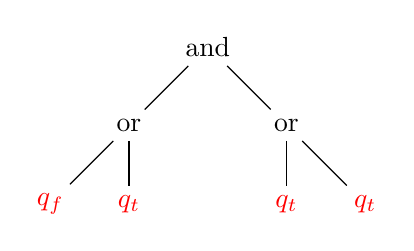
\begin{tikzpicture}[auto]
	\node (and) at (2, 3) {and};
	\node (or1) at (1, 2) {or};
	\node (or2) at (3, 2) {or};
	\node (false1) at (0, 1) {\textcolor{red}{$q_f$}};
	\node (true1) at (1, 1) {\textcolor{red}{$q_t$}};
	\node (true2) at (3, 1) {\textcolor{red}{$q_t$}};
	\node (true3) at (4, 1) {\textcolor{red}{$q_t$}};
	
	\draw [-] (and) to (or1);
	\draw [-] (and) to (or2);
	\draw [-] (or1) to (false1);
	\draw [-] (or1) to (true1);
	\draw [-] (or2) to (true2);
	\draw [-] (or2) to (true3);
	\end{tikzpicture}
	\\
	\centering \(false\) and \(true,\) \textit{according to our initial rules, are reduced to} \(q_f\) \textit{and} \(q_t\).
\end{minipage}
\\
\\
\\
\begin{minipage}{0.5\textwidth}
		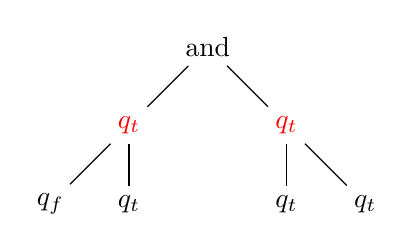
\begin{tikzpicture}[auto]
		\node (and) at (2, 3) {and};
		\node (or1) at (1, 2) {\textcolor{red}{$q_t$}};
		\node (or2) at (3, 2) {\textcolor{red}{$q_t$}};
		\node (false1) at (0, 1) {$q_f$};
		\node (true1) at (1, 1) {$q_t$};
		\node (true2) at (3, 1) {$q_t$};
		\node (true3) at (4, 1) {$q_t$};
		
		\draw [-] (and) to (or1);
		\draw [-] (and) to (or2);
		\draw [-] (or1) to (false1);
		\draw [-] (or1) to (true1);
		\draw [-] (or2) to (true2);
		\draw [-] (or2) to (true3);
		\end{tikzpicture}
	\\
	\centering \(or(q_f, q_t)\) \textit{and} \(or(q_t, q_t)\) \textit{are reduced to} \(q_t\) \textit{each.}
\end{minipage}
\begin{minipage}{0.5\textwidth}
	~~
	\begin{tikzpicture}[auto]
	\node (and) at (2, 3) {\textcolor{red}{$q_t$}};
	\node (or1) at (1, 2) {$q_t$};
	\node (or2) at (3, 2) {$q_t$};
	\node (false1) at (0, 1) {$q_f$};
	\node (true1) at (1, 1) {$q_t$};
	\node (true2) at (3, 1) {$q_t$};
	\node (true3) at (4, 1) {$q_t$};
	
	\draw [-] (and) to (or1);
	\draw [-] (and) to (or2);
	\draw [-] (or1) to (false1);
	\draw [-] (or1) to (true1);
	\draw [-] (or2) to (true2);
	\draw [-] (or2) to (true3);
	\end{tikzpicture}
	\\
	\centering \(and(q_t, q_t)\) \textit{is reduced to} \(q_t\).
	\\~
\end{minipage}
\\
\\
\begin{center}
	\begin{tikzpicture}[auto]
	\node (and) at (2, 3) {$q_t$};
	\node (or1) at (1, 2) {$q_t$};
	\node (or2) at (3, 2) {$q_t$};
	\node (false1) at (0, 1) {$q_f$};
	\node (true1) at (1, 1) {$q_t$};
	\node (true2) at (3, 1) {$q_t$};
	\node (true3) at (4, 1) {$q_t$};
	
	\draw [-] (and) to (or1);
	\draw [-] (and) to (or2);
	\draw [-] (or1) to (false1);
	\draw [-] (or1) to (true1);
	\draw [-] (or2) to (true2);
	\draw [-] (or2) to (true3);
	\end{tikzpicture}
	\\
	\centering \textit{The final stage.}
	\\~
\end{center}

In this graphical representation we kept the states after reducing them. However, this is not needed for running an automaton like the formal version of this run shows:\\\\
\(and(or(false, true), or(true, true)) \moveStar and(or(q_f, q_t), or(q_t, q_t)) \\ \moveStar and(q_t, q_t) \moveStar q_t \)\\\\
Since the tree could be reduced to the accepting state \(q_t \in Q_f\), we can say that \(A\) accepts \(w\) and therefore the tree \(w\) is in the language \(L_A\) recognized by the automaton.
\\
\\
\end{example}

\chapter*{Determinization}

Non Deterministic Finite Tree Automata (NFTA) can be determinized just like Non Determinitistic Automata (NFA) in the word case. By knowing that there exists a DFTA for every NFTA, definitions, proofs and algorithms become much easier, since we don't have to take special care of the properties of NFTAs. We will now take a look at how this is done. But first we have to define formally, what being deterministic means in the context of FTAs.

\begin{definition}{Deterministic Finite Tree Automaton}

	A tree automaton with no two rules of the type:
	\begin{center}
		\(f(q_1,..., q_n) \rightarrow q_x\)\\
		\(f(q_1,...,q_n) \rightarrow q_y\)\\
		with \(q_x \neq q_y\) \\
	\end{center}
	or
	\begin{center}
		\(\epsilon(q_1, ..., q_n) \rightarrow q_x\)\\
		(state changes, even though no actual symbol is read)
	\end{center}
	with \(n \ge 0, q_x,q_y,q_1,...q_n \in Q, q_x \neq q_y, f \in \Sigma\)
	is called a \textbf{Deterministic Finite Tree Automaton} (DFTA).
\end{definition}

Similar to the algorithm for Determinization in the word case, there exists a power set construction algorithm for determizing Tree Automata.

\begin{definition}{Algorithm DET for Tree Automata \cite{tata-nfta}}\\
	Note: statesOf(x) returns the set of states that contributed to the creation of the state x, while state(X) returns a state representing all states in the set X.
\begin{algorithm}[H]
	\KwData{NFTA \(A = (Q, \Sigma, Q_f ,\Delta)\)}
	\(Q_d := \emptyset\)\\
	\(\Delta_d := \emptyset\)
	\\
		\While{\(\Delta_d\) grew last cycle} {
			\( f(q_1,...,q_n) \in \Delta\)\\
			\(s_1,...,s_n \in Q_d\)\\
			~\\
			/* meta-state representing the set of reachable states */ \\
			\( s := state(\{ q \in Q ~|~ q_1 \in statesOf(s_1),..., q_n \in statesOf(s_n), f(q_1,...q_n) \rightarrow q \in \Delta \}) \)\\~\\
			\(Q_d := Q_d \cup \{s\}\)\\
			\(\Delta_d := \Delta_d \cup f(s_1,...,s_n) \rightarrow s \)
		}
	\(Q_{f_d} := \{ s \in Q_d ~ | ~ \{s\} \cap Q_d \neq \emptyset \}\)\\
	\KwResult{DFTA \(A_d = (Q_d, \Sigma, Q_{f_d}, \Delta_d) \)}
\end{algorithm}
\end{definition}

\pagebreak

It is easy to see that the algorithm produces a deterministic automaton \(A_d\) as we are automatically constructing meta-states for all reachable states and therefore eliminating all possible non-deterministic behaviour. However, we still have to prove \(L(A) = L(A_d)\). For this, we have to show that the meta-states \(s \in Q_d\) are "built correctly", or in formal terms:

\begin{center}
	\(For~any~tree~t: t \moveStarDet s \iff s = state(\{q \in Q ~|~ t \moveStar q\})\)
\end{center}


\begin{proof}{\(L(A) = L(A_d)\) (Correctness of DET) \cite{tata-nfta}}\\
	This proof is done via an induction over the structure of the symbols in \(\Sigma\).
	\begin{itemize}
		\item \textbf{Base case:}
			For any tree \(t = a \in \Sigma\) we take a look at the rule \(a \rightarrow q(a)\). Because of the way we defined \(s\) as the meta-state representing the set of all reachable states in a given situation this is inherently correct.
			\\
		\item \textbf{induction step: \(t = f(q_1,... , q_n)\)}
			\begin{itemize}
				\item 
				1.: \(t \moveStarDet s \Rightarrow (s = state(\{q \in Q ~|~ t \moveStar q\})\)\\\\
				Supposing \(t \moveStarDet f(s_1, ..., s_n) \rightarrow_{A_d} s\), by induction hypothesis, for each \(i \in {1,..., n}\), we can see \(s_i = state(\{q \in Q ~|~ q_i \moveStar q\}\).\\
				\\
			    Because states \(s_i \in Q_d\), rules \(f(s_1, ..., s_n) \rightarrow s \in \Delta_d\) are added by the determinization algorithm and \( s := state(\{ q \in Q ~|~ q_1 \in statesOf(s_1),..., q_n \in statesOf(s_n), f(q_1,...q_n) \rightarrow q \in \Delta \}) \), we learn \(s = state(\{q \in Q ~|~ t \moveStar q\})\).
				\\
				\item
				2.: \(s = state(\{q \in Q ~|~ t \moveStar q\}) \Rightarrow t \moveStarDet s\)\\\\
				Considering \(s = state(\{q \in Q ~|~ f(q_1, ..., q_n) \moveStar q\})\) with state sets \(S_i\) defined as \(S_i := \{q \in Q ~|~ q_i \moveStar q\}\), by induction hypothesis for each \(i \in \{1, ..., n\}\) we know \(q_i \moveStarDet s_i, s_i = state(S_i)\).
				Thus \( s = state(\{ q \in Q ~|~ q_1 \in S_1,..., q_n \in S_n, f(q_1,...q_n) \rightarrow q \in \Delta \}) \).\\
				\\
				By the definition of \(\Delta_d\) in the determinization algorithm, \(f(s_1, ..., s_n) \in \Delta_d\) and thus \(t \moveStarDet s\).
			\end{itemize}
	\end{itemize}
	\qed
\end{proof}

\pagebreak

\newcommand{\automatonDefinition} {
	\(A = (Q, \Sigma, Q_f, \Delta)\)
}

Following is an example of how a NFTA can be determinized with this algorithm.

	\begin{example}{Running the DET algorithm}
		\\
		consider a non deterministic FTA given like this:\\
		\automatonDefinition\\
		\(\Sigma = \{ul, li, text, empty\}\)\\
		\(Q = \{q_{ul}, q_{li1}, q_{li2}, q_{text}, q_{empty}\}\)\\
		\(Q_f = \{q_{ul}\}\)\\
		\(\Delta = \{
		ul(q_{li1},q_{li2}) \rightarrow q_{ul}, ul(q_{li2},q_{li1}) \rightarrow q_{ul}, \newline
		\mathbf{li(q_{text}) \rightarrow q_{li1}, li(q_{text}) \rightarrow q_{li2},}\newline
		text \rightarrow q_{text}, empty \rightarrow q_{empty}, \newline
		\mathbf{\epsilon(q_{empty}) \rightarrow q_{text}}
		\}\)
		\\\\
		This recognizes all trees that represent unordered lists (ul) in HTML notation, which contain 2 list items (li):
			%careful: space indentation
			\lstset{
				basicstyle=\footnotesize, frame=tb,
				xleftmargin=.4\textwidth, xrightmargin=.5\textwidth
			}
			\begin{lstlisting}[frame=none]
<ul>
    <li>text</li>
    <li>empty</li>
</ul>
			\end{lstlisting}
			Or as a tree input:
			\begin{center}
				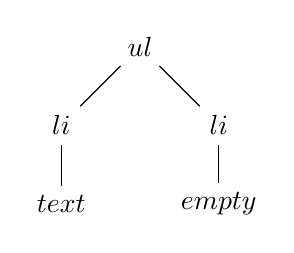
\begin{tikzpicture}[auto]
				\node (and) at (2, 3) {$ul$};
				\node (or1) at (1, 2) {$li$};
				\node (or2) at (3, 2) {$li$};
				\node (true1) at (1, 1) {$text$};
				\node (true2) at (3, 1) {$empty$};
				
				\draw [-] (and) to (or1);
				\draw [-] (and) to (or2);
				\draw [-] (or1) to (true1);
				\draw [-] (or2) to (true2);
				\end{tikzpicture}
			\end{center}
					If we start determinizing with the rules containing no state and then go "up in the hierarchy" and generate all the states on-the-fly, we get these new rules:
					\\
					\(
					\newline
					text \rightarrow state(\{q_{text}\})
					\newline
					empty \rightarrow state(\{q_{text}, q_{empty}\})\)
					\\
					\(li(state(\{q_{text}\}))) \rightarrow state(\{q_{li1}, q_{li2}\})\)
					\newline
					\(li(state(\{q_{text}, q_{empty}\})) \rightarrow state(\{q_{li1}, q_{li2}\})
					\newline
					ul(state(\{q_{li1}, q_{li2}\}), state(\{q_{li1}, q_{li2}\})) \rightarrow state(\{q_{ul}\})
					\)
					\\
					\\
				    And the set of final states is \(Q_{f_d} = \{state(\{q_{ul}\})\}\).
				    \\
				    \\
				    As we can see, there is no \(\epsilon\)-rule left and we don't have to choose which rule to apply when reading 
			\end{example}

\pagebreak

\chapter*{Minimization}

Now that we can obtain a DFTA for each NFTA, we can take a look at how we can minimize these newly determinized automata.
\\
Just like in the word case there exists a Myhill-Nerode theorem for Finite Tree Automata. But before we can use it, we have to define \textbf{Contexts}, \textbf{Congruence} and \(\equiv_L\).
\\\\
For the definition of a \textbf{Context} it is convenient to define a \textbf{Slot} first.

\begin{definition}{Slot} \textcolor{red}{(is this definition sufficient?)}\\
	A \textbf{Slot} \(s \in S, S \cap \Sigma = \emptyset\) is a special token, that, if found in a tree \(t_1 \in T_{\Sigma \cup S}\), can be replaced by any tree \(t_1 \in T_{\Sigma \cup S}\) (\(t_2\) can contains \textbf{slots} as well).
\end{definition}
~\\
As an abstract representation, a tree with a slot is often drawn as a triangle with a marker for every slot:
\\\\
\begin{minipage}{0.5\textwidth}
	\begin{center}
		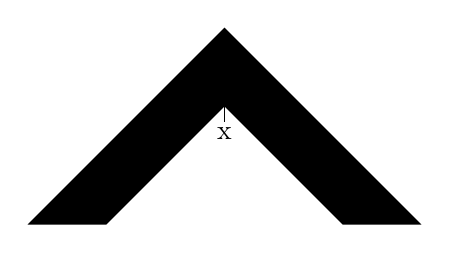
\begin{tikzpicture}
		\fill[black] (-0.5, -0.5) -- (0.5, -0.5) -- (2, 1) -- (3.5, -0.5) -- (4.5, -0.5) -- (2, 2) -- (-0.5, -0.5);
		\draw[black] (2, 1) -- (2, 0.8);
		\node at (2, 0.65) {x};
		\end{tikzpicture}
		\captionof{figure}{Tree with the slot \(x\) \cite{martens-uni-dortmund-lecture01}}
	\end{center}
\end{minipage}
\begin{minipage}{0.5\textwidth}
	\begin{center}
		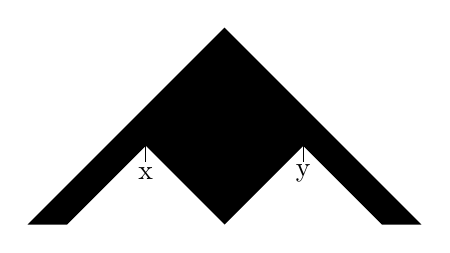
\begin{tikzpicture}
		\fill[black] (-0.5, -0.5) -- (0, -0.5) -- (1, 0.5) -- (2, -0.5) -- (3, 0.5)  -- (4.0, -0.5) -- (4.5, -0.5) -- (2, 2) -- (-0.5, -0.5);
		\draw[black] (1, 0.5) -- (1, 0.3);
		\node at (1, 0.15) {x};
		\draw[black] (3, 0.5) -- (3, 0.3);
		\node at (3, 0.15) {y};
		\end{tikzpicture}
		\captionof{figure}{Tree with the slots \(x\) and \(y\) \cite{martens-uni-dortmund-lecture01}}
	\end{center}
\end{minipage}
~\\\\
Defining a Context is straightforward now.

\begin{definition}{Context} \cite{tata-nfta}\cite{martens-uni-dortmund-lecture01}\\
	A tree with slots is called a \textbf{Context}. Furthermore, if \(C\) is a context with slots \(s_1, ..., s_n \in S\), then \(C[t_1, ..., t_n], t_1, ..., t_n \in T_\Omega\) is known as a \textbf{context application}, with the slots \(s_i\) being replaced by (sub-)trees \(t_i \in T_\Omega, T_\Omega \supseteq T_{\Sigma \cup S}\).
	\\\\
	Note: \(T_\Omega\) \textbf{can} contain new slots.
	\\\\
\end{definition}
\begin{minipage}{0.5\textwidth}
	\begin{center}
		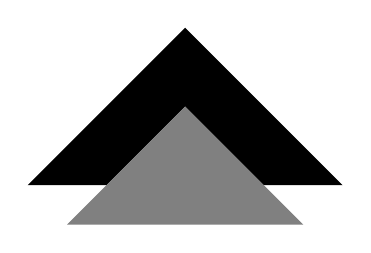
\begin{tikzpicture}
		\fill[black] (0,0) -- (1, 0) -- (2, 1) -- (3, 0) -- (4, 0) -- (2, 2) -- (0,0);
		\fill[gray] (0.5, -0.5) -- (3.5, -0.5) -- (2, 1) -- (0.5, -0.5);
		\end{tikzpicture}
		\captionof{figure}{Context application \cite{martens-uni-dortmund-lecture01}}
	\end{center}
\end{minipage}
\begin{minipage}{0.5\textwidth}
	\begin{center}
		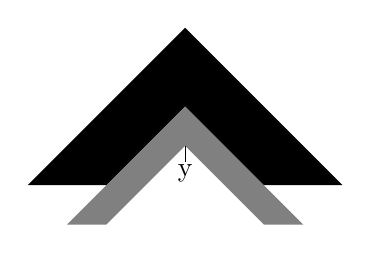
\begin{tikzpicture}
		\fill[black] (0,0) -- (1, 0) -- (2, 1) -- (3, 0) -- (4, 0) -- (2, 2) -- (0,0);
		\fill[gray] (0.5, -0.5) -- (1, -0.5) -- (2, 0.5) -- (3.0, -0.5) -- (3.5, -0.5) -- (2, 1) -- (0.5, -0.5);
		\draw[black] (2, 0.5) -- (2, 0.3);
		\node at (2, 0.15) {y};
		\end{tikzpicture}	
		\captionof{figure}{Context application with a new context \cite{martens-uni-dortmund-lecture01}}
	\end{center}
\end{minipage}

\begin{definition}{Congruence} \cite{tata-nfta} \\
	An equivalence relation \(\equiv\)  on \(T_\Sigma\) is a \textbf{congruence} on \(T_\Sigma\) if for every \(f \in \Sigma\) with \(n\) arguments applies:
	\begin{center}
		\(T_\Sigma \ni u_i \equiv w_i \in T_\Sigma, 1 \leq i \leq n \Rightarrow f(u_1, ..., u_n) \equiv f(w_1, ..., w_n)\)\\
		\(\#~of \equiv-classes~is~finite \Rightarrow \equiv\) is of \textbf{finite index}.
	\end{center}
	Additionally a congruence is an equivalence relation closed under context. This means that for any \(C \in T_{\Sigma \cup V}\), if \(u \equiv w \Rightarrow C[u] \equiv C[w]\).
\end{definition}

\begin{definition}{\(\equiv_L\)} \cite{tata-nfta} \\
	For any given tree language \(L \in T_\Sigma\), we define the congruence \(\equiv_L\) on \(T_\Sigma\) by: \(T_\Sigma \ni u \equiv_L w \in T_\Sigma\), if for all Contexts \(C \in T_{\Sigma \cup V}\) applies:
	\begin{center}
		\(C[u] \in L \iff C[v] \in L\)
	\end{center}
\end{definition}

For the sake of easier proofs, we consider all following DFTAs to be \textbf{complete} and \textbf{reduced}.

\begin{definition}{Completeness and reduction} \cite{wiki-tree-automaton}\\
A FTA A is \textbf{complete} if there is at least one transition rule available for every possible symbol-states combination. A state \(q\) is \textbf{accessible} if there exists a tree \(t\) such that \(t \moveStar q\). A NFTA is \textbf{reduced} if all its states are accessible.
\end{definition}

\textit{Note: All examples for Finite Tree Automata given in this paper are supposed to be complete and reduced. However, we do not add a capturing state for all impossible symbol-state combinations for the sake of simplicity. Let \(q_c \in Q\) be the capturing state, then every transition rule that contained it state on the left side look like \(f(..., q_c, ...) \rightarrow q_c\). This means, that once the capturing state is reached, there is no way of getting to a different state anymore.}

\pagebreak

We can now give the Myhill-Nerode theorem.

\begin{theorem}{Myhill-Nerode} \cite{tata-nfta}\\
	These statements are equivalent:\\\\
	(i) \(L\) is a regular tree language\\\\
	(ii) \(L\) is the union of some congruence classes of finite index\\\\
	(iii) the relation \(\equiv_L\) is a congruence of finite index
\end{theorem}

\begin{proof}{~}
	\begin{itemize}
		\item (i) \(\Rightarrow\) (ii): Assume that the tree language \(L\) is recognized by some complete DFTA \(A = (Q, \Sigma, Q_f, \delta)\) with \(\delta\) being a transition function (i).
		Let us consider the relation \(\equiv_A\) defined on \(T_\Sigma\) by: \(T_\Sigma \ni u \equiv v \in T_\Sigma\), if \(\delta(u) = \delta(v)\). Since we know that \(Q\) only has a finite amount of states in it and the number of equivalence classes may at most be equal to the size of \(Q\), we can deduce that \(\equiv_A\) is a congruence of finite index (ii).
		\\
		\item (ii) \(\Rightarrow\) (iii): By denoting the congruence of finite index as \(\cong\) and assuming that \(T_\Sigma \ni u \cong v \in T_\Sigma\), it can be proven that \(C[u] \cong C[v]\) for all contexts \(C \in T_{\Sigma \cup V} \) by an easy induction on the structure of terms. Since \(L\) is the union of some equivalence classes of the congruence of finite index \(\cong\) (ii), we have \(C[u] \in L \iff C[v] \in L \). Therefore we know that  \( u \equiv_L v \) and that \( \equiv_L \) contains the equivalence class of u in \( \cong \). Furthermore we now know that \(index(\equiv_L) \leq index(\cong) \Rightarrow index(\equiv_L)~is~finite \) (iii).
		\\
		\item (iii) \(\Rightarrow\) (i):
		 By representing the set of equivalence classes of \( \equiv_L \) (iii) as the finite set of states \(Q_{min}\) with \(|Q_{min}| = |\equiv_L|\), we know that every equivalence class has its own state. By denoting the equivalence class of a term \(u \in T_\Sigma\) as \([u]\) we define the transition function \(\delta_{min}\) for every \( f \in \Sigma\) with \(n\) arguments as:
		 \begin{center}
			 \(\delta_{min}(f, [u_1], ..., [u_n]) = [f(u_1, ..., u_n)]\)
		 \end{center}
		 The definition of \(\delta\) is consistent because \(\equiv_L\) is a congruence. With \(Q_{min_f} := \{ [u] | u \in L \}\) the resulting DFTA \(A_{min} := (Q_{min}, \Sigma, Q_{min_f}, \delta_{min}\) recognizes the tree language \(L\) (i). 
		 \qed
	\end{itemize}
\end{proof}

\pagebreak

As a consequence of this theorem we can deduce the following:

\begin{corollary} \cite{tata-nfta}\\
	The minimum DFTA recognizing a tree language \(L\) is unique up to renaming the states and is given by \(A_{min}\) in the proof of the Myhill-Nerode Theorem.
\end{corollary}

This means that we can minimize a tree automaton by computing the congruence classes of the language it recognizes. But before we can put this to use, we have to prove the corollary first.

\begin{proof} {~} \cite{tata-nfta}\\
	Assume that \(L\) is recognized by some DFTA \(A = (Q, \Sigma, Q_f, \delta)\). Then the relation \(\equiv_A\) is a refinement of \(\equiv_L\) with \(index(\equiv_A) \geq index(\equiv_L)\), thus \(|Q| \geq |Q_{min}|\). We know that \(A\) is reduced (all states are accesible), because otherwise a state could be removed contradicting to the definition of \(\equiv_A\). Let \(q \in Q\) and \(u \in T_\Sigma\), such that \(\delta(u) = q\). Then the state \(q\) can be consistently identified with the state \(\delta_{min}(u)\), since \(\delta\) is a refinement of \(\delta_{min}\) and we can see that every state \(q \in Q\) has a corresponding state \(q_{min} \in Q_{min}\).
	\qed
\end{proof}

By using this Corollary and the construction given in the Myhill-Nerode theorem we can deduce an algorithm to minimize Deterministic Finite Tree Automata:

\begin{definition}{Algorithm MIN for Tree Automata} \cite{martens-uni-dortmund-lecture02}\\
	\begin{algorithm}[H]
		\KwData{complete and reduced DFTA \(A = (Q, \Sigma, Q_f ,\Delta)\)}
		Set \(P = \{(q_f, q)~|~q_f \in Q_f, q \in Q \setminus Q_f\}\)\\
		Set \(P' = P\)\\
		\While{\(P' \neq P\)} {
			\(P = P'\)\\
			\(\forall p_1, p_2, p_3 \in Q, p_1 \neq p_2, p_1 \neq p_3, p_2 \neq p_3,\)\\
			define \(\neg (p_1P'p_2) \iff\)\\
			~~~~/* coudln't distinguish to anything in the last cycle */\\
			\textcolor{red}{ist das hier \(p_3\)? Weil sonst bricht das ja sofort ab...}\\
			~~~~1.\(\neg(p_1Pp_3)\) or\\
			~~~~/* can't distinguish \(p_1\) from \(p_2\), yet */\\
			~~~~2.\(\exists f \in \Sigma\) with \(n\) arguments, \(\exists q_1, ..., q_{i-1}, q_{i+1}, ..., q_n \in Q\), \\
			~~~~~ \(\neg(r_1Pr_2), r_1, r_2 \in Q\), where: \\
			~~~~~~~ \(f(q_1, ..., q_{i-1}, p_1, q_{i+1}, ..., q_n) \rightarrow r_1\) and\\
			~~~~~~~ \(f(q_1, ..., q_{i-1}, p_2, q_{i+1}, ..., q_n) \rightarrow r_2\) \\
			~~~~~~~ (Note: this works for multiple occurences of \(p_1\) and \(p_2\) as well, \\
			~~~~~~~~ see the example on the next page)
		}
		\(Q_{min} = \) set of equivalence classes of P \\
		\(\Delta_{min} = \{f([q_1], ..., [q_n]) \rightarrow [q]~|~f(q_1, ..., q_n) \rightarrow q \in \Delta\}\)\\
		\(Q_{f_{min}} = \{[q]~|~q \in Q_f\}\)\\
		\KwResult{complete, reduced and minimal DFTA \(A_{min} = (Q_{min}, \Sigma, Q_{f_{min}}, \Delta_{min}) \)}
	\end{algorithm}
\end{definition}

\pagebreak


While we are not giving a complete proof for this algorithm, we can at least go over why it is correct for a given language \(L = L(A)\) and the automaton \(A = (Q, \Sigma, Q_f, \Delta) \) \cite{tata-nfta}:
\begin{itemize}
	\item In the while loop we are marking all tuples \(p_1, p_2\) as distinguishable when they are added to the relation
	\\
	\item In order to get the equivalence classes for \(Q_{min}\), we are merging all pairs of indistinguishable states to a new one representing both. After having done this incrementally for all not marked combinations, these "artificial" states have to be distinguishable to all other states and \(Q_{min}\) must therefore be minimal. This can easily be proven correct by contradiction.
	\\
	\item It isn't hard to see that the construction of \(Q_{f_{min}}\) and \(\Delta_{min} \) is correct.
\end{itemize}

\begin{example}{Running the MIN algorithm}\\
After cleaning up the Automaton of our previous unordered list example, one might already see that it isn't minimal yet:\\\\
				\automatonDefinition
				\(\Sigma = \{ul, li, text, empty\}\)
				\\
				\(Q = \{q_{ul}, \mathbf{q_{text}, q_{text2}}, q_{li}\}\)
				\\
				\(Q_f = \{ q_{ul} \}\)
				\\
				\(\Delta = \{		text \rightarrow q_{text},
				\newline
				empty \rightarrow q_{text2},
				\newline
				\mathbf{
					li(q_{text}) \rightarrow q_{li},	
				}	
				\newline
				\mathbf {
					li(q_{text2}) \rightarrow q_{li},
				}
				\newline
				ul(q_{li}, q_{li}) \rightarrow q_{ul}
				\}\)
				\\
				\\
While we should be able to fix this by hand, we are now using the MIN algorithm to minimize this automaton. In the following table, we are marking all tuples \(p_1, p_2\) that are distinguishable in that cycle by the index of that cycle, so we can see the process in action.
\begin{center}
	\begin{tabular}{| l |  l | l | l |  l  |}
		\hline
		&	 \(q_{text}\) 	& 	\(q_{text2}\) 	& 	\(q_{li}\)  	& 	\(q_{ul}\) 	\\ \hline
		\(q_{text}\) 	&	-			&	-			&	-		&	-		\\ \hline
		\(q_{text2}\) 	&	(merge)	&	-		&	-		&	-		\\ \hline
		\(q_{li}\) 		&	1			&	1			&	-		&	-		\\ \hline
		\(q_{ul}\) 		&	0			&	0			&	0		&	-		\\
		\hline
	\end{tabular}
\end{center}

\pagebreak

As predicted \(q_{text}\) and \(q_{text2}\) have to be merged in order to minimize \(A\). The resulting automaton is:
\\
\\
\automatonDefinition
\(\Sigma = \{ul, li, text, empty\}\)
\\
\(Q = \{q_{ul}, \mathbf{q_{text_{1\&2}}}, q_{li}\}\)
\\
\(Q_f = \{ q_{ul} \}\)
\\
\(\Delta = \{		text \rightarrow \mathbf{q_{text_{1\&2}}},
\newline
empty \rightarrow \mathbf{q_{text_{1\&2}}},
\newline
\mathbf{
	li(q_{text_{1\&2}}) \rightarrow q_{li},	
}
\newline
ul(q_{li}, q_{li}) \rightarrow q_{ul}
\}\)
\\
\\
\end{example}

\pagebreak

%
% ---- Bibliography ----
%
\begin{thebibliography}{99}
%
\bibitem {automata-xml}
	Automata theory for XML researchers,
	Frank Neven,
	University of Limburg,
	frank, neven~luc, ac. be,
	\url{http://homepages.inf.ed.ac.uk/libkin/dbtheory/frank.pdf}, 03/11/2015
\bibitem {tata-nfta}
	Tree Automata and Techniques, Hubert Comon et. al, Pages 19-39
\bibitem {martens-uni-dortmund-lecture01}
	Automata and Logic on Trees,
	Wim Martens,
	Stijn Vansummeren,
	\url{http://lrb.cs.uni-dortmund.de/\textasciitilde martens/data/esslli07/lecture01.pdf}, 03/17/2015
\bibitem {martens-uni-dortmund-lecture02}
	Automata and Logic on Trees,
	Wim Martens,
	Stijn Vansummeren,
	\url{http://lrb.cs.uni-dortmund.de/\textasciitilde martens/data/esslli07/lecture02.pdf}, 03/21/2015
\bibitem {wiki-tree-automaton}
	\url{http://en.wikipedia.org/wiki/Tree\_automaton}, 03/20/2015




\end{thebibliography}

\end{document}
